\section{Factorial StateBind}
\label{sec:method}

Oracle Physicalized uses human geometry. An automatic verifier must instead estimate the target state and the value--scale mapping from the image, while recognizing when those estimates support a stable choice. The pipeline has three steps: factor two proposals into target and lattice components, verify each component once, and accept only choices invariant to exchanging component sources.

\subsection{Propose, Canonicalize, and Validate}

Two VLM proposers $D$ and $G$ receive only $(I,q,\C)$. We write response $r$ as $P_r=(T_r,L_r,o_r)$: target geometry, a local scale lattice (axis, ticks, anchors, tick value, unit, branch, and direction), and its readout operator. Coordinates use a normalized $[0,1000]^2$ frame and are rescaled to native pixels.

The proposer orients axis direction $\vect u$ toward increasing values. Projection onto $\vect u$ signs $\delta_p$ numerically. From projected ticks $p_k$, anchors $(p_a,v_a)$, and minor-tick value $\delta_v$, the local map is
\begin{equation}
 \delta_p=\operatorname{median}_k(p_{k+1}-p_k),\quad
 \phi=\operatorname{median}_a\!\left(p_a-\frac{v_a}{\delta_v}\delta_p\right),\quad
 \hat p(v)=\phi+\frac{v}{\delta_v}\delta_p .
 \label{eq:auto-map}
\end{equation}
Unit conversion is deterministic. Qwen acts as an independent component verifier: it inspects rendered target, anchor, lattice, branch, and operator evidence but does not output an A/B candidate. A proposal is executable when the required components are visually supported, tick spacing is positive, units are compatible, and the target and lattice use the same operator. Human geometry and evaluator answers are not inputs to this process.

\subsection{Cross-Source Recombination}

The two proposals yield four target--lattice combinations,
\begin{equation}
 \Hset=\{(T_D,L_D),(T_D,L_G),(T_G,L_D),(T_G,L_G)\}.
 \label{eq:factorial}
\end{equation}
Combination $(T_i,L_j)$ is executable only when both components pass validation and $o_i=o_j$. Let $\hat z_{ij}=\Psi_{o_i}(T_i,L_j)$ be the reading obtained by interpreting target $T_i$ in lattice $L_j$ under their shared operator. For a single-state task, $\Psi$ maps the target interval through $L_j$; for a span, it returns the absolute difference between the two mapped endpoints. Invalid combinations are omitted. Every valid combination deterministically selects
\begin{equation}
 \hat c_{ij}=\arg\min_{c\in\C}\R(c;\hat z_{ij}),\qquad
 \rho(c)=\frac{\sum_{(i,j)\in\Hset_{\rm valid}}\mathbf{1}[\hat c_{ij}=c]}
 {|\Hset_{\rm valid}|},
 \label{eq:choice}
\end{equation}
where $\R$ is distance from a candidate to a single-state interval or to the estimated endpoint difference. The method therefore changes which source supplies the target and lattice without asking a VLM to make four new holistic guesses.

\begin{figure}[t]
  \centering
  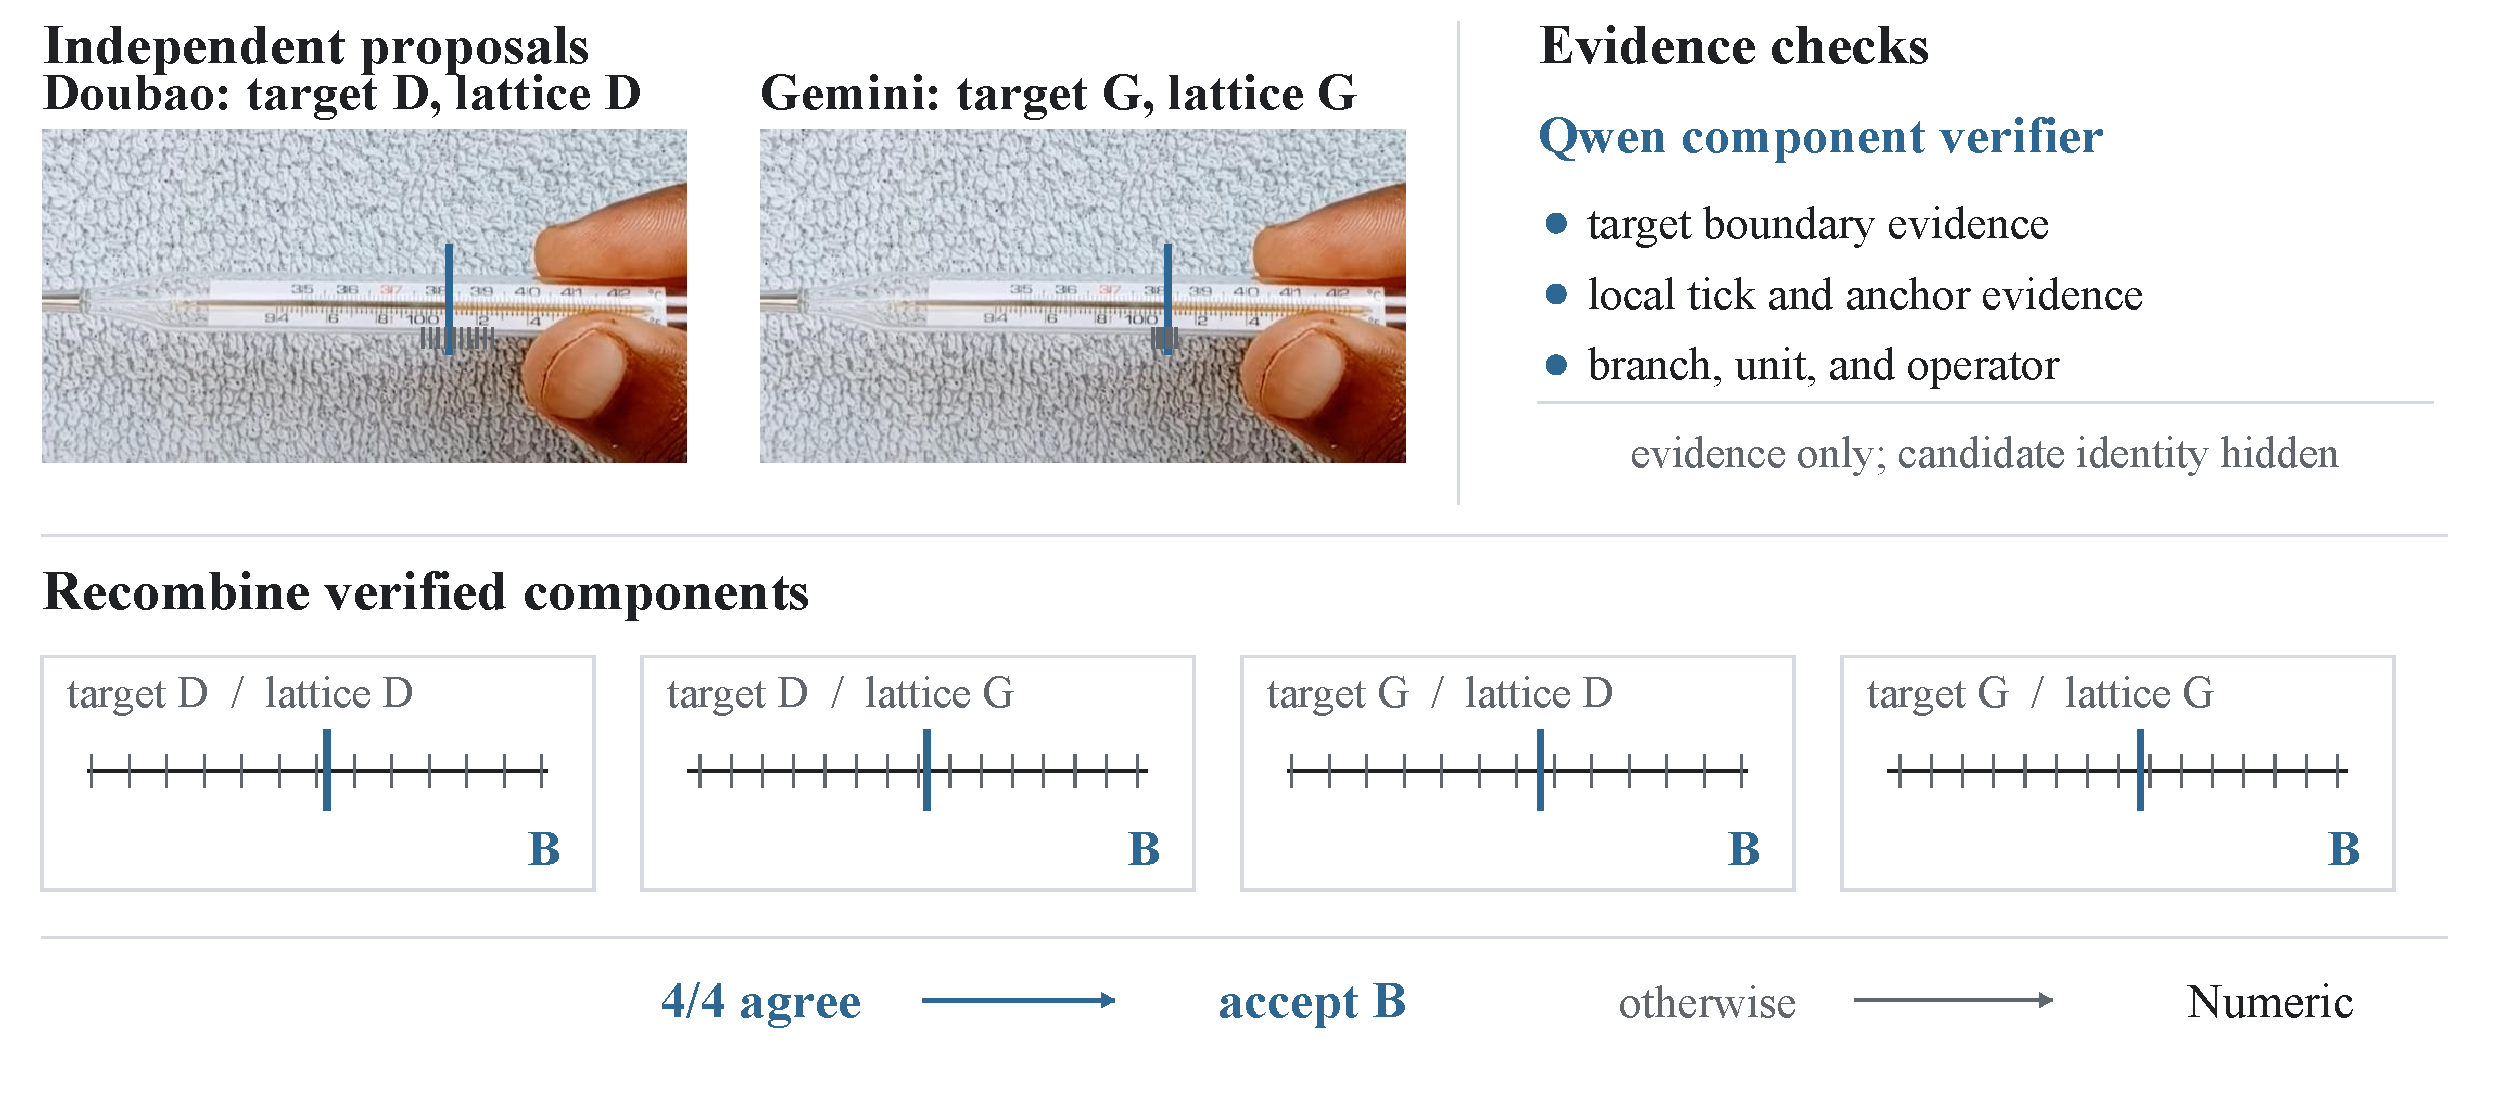
\includegraphics[width=\textwidth]{fig4_factorial_architecture.pdf}
  \caption{\textbf{Factorial StateBind.} Doubao and Gemini independently propose target and lattice components. Qwen verifies their visual evidence. The four valid target--lattice source combinations are resolved deterministically; agreement defines candidate support, while disagreement triggers the Numeric fallback. Precision mode accepts four-source agreement with adequate state separation. Source image: MeasureBench~\cite{lin2026measurebench}, CC BY-SA 4.0; cropped and annotated by the authors.}
  \label{fig:architecture}
\end{figure}

\subsection{Precision Mode}

The general method exposes component validity, candidate support $\rho$, state separation, and dispersion. Let $\Delta_{\C}=|c_1-c_2|/\delta_v$ denote candidate separation in local ticks. For this benchmark we predefine nine selective rules on Dev69: three agreement requirements (4/4; unanimous over at least three valid combinations; three-of-four majority), crossed with minimum separations of 1, 2, and 4 ticks. Maximum coverage subject to at least 95\% development precision selects
\begin{equation}
 |\Hset_{\rm valid}|=4,\qquad \rho(\hat c)=1,\qquad
 \Delta_{\C}\ge4~\text{ticks}.
 \label{eq:precision}
\end{equation}
This precision mode routes 50 of 414 development ordered cells at 98.00\% precision and is applied unchanged to Paired128; cells not routed retain their Numeric reader. Across 20,000 source-image bootstrap samples, the four-way agreement family is selected in \FourWayFamilyBootstrapSelection\% of replicates, and the frozen four-tick rule satisfies the 95\% precision requirement in \FrozenRuleBootstrapFeasible\%. The winning separation varies among one, two, and four ticks, identifying four-source agreement as the stable rule family and four ticks as its high-precision operating point.

Self agreement uses $(T_D,L_D)$ and $(T_G,L_G)$ and can preserve a target--lattice displacement shared within each proposal. The off-diagonal pairs $(T_D,L_G)$ and $(T_G,L_D)$ break that coupling. Full recombination retains both views and asks whether the final candidate is stable across every component source.
